\documentclass[a4paper,12pt]{article}
\usepackage[russian]{babel}
\usepackage[utf8]{inputenc}
\usepackage[hidelinks]{hyperref}
\usepackage{amssymb}
\usepackage{amsmath}
\usepackage{graphicx}
\graphicspath{{/}}
\DeclareGraphicsExtensions{.pdf,.png,.jpg}

\begin{document}
\section*{17. Способы борьбы с переобучением. Байесовская сеть доверия: определение и применение. Уменьшение размерности пространства признаков.}
\url{http://logic.pdmi.ras.ru/csclub/sites/default/files/slides/20080330_machine_learning_nikolenko_lecture07.pdf}
\url{http://www.habarov.spb.ru/new_es/exp_sys/es06/es6.htm}
\url{https://class.coursera.org/pgm/lecture/3}

\subsection*{Способы борьбы с переобучением}

TBD.

\subsection*{Байесовская сеть доверия}
\textit{Байесовская сеть} -- графическая вероятностная модель, представляющая собой множество переменных и их вероятностных зависимостей. Является в некотором роде продолжением байесовского классификатора. Б.К. основывается на предположении об условной независимости атрибутов при условии данного целевого значения. Б.С. представляет собой направленный граф, в котором стрелки показывают причинно-следственную связь. В вершинах графа заданы условные вероятности при условии всего множества предков. Если предков нет, вероятности не условные, а маргинальные. В графе запрещены направленные циклы. Вся эта информация дает возможность вычислять любую вероятность в сети, т.е. единственным образом задает распределение.

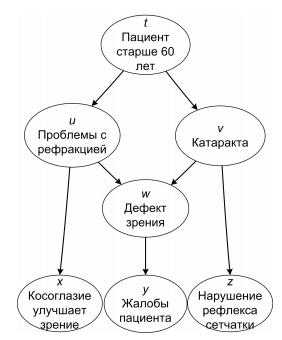
\includegraphics{network}

Суть рассуждений в байсовской сети -- пропагация свидетельств. Обычно пропагация идёт снизу вверх, от следствий к причинам.

\textbf{Теорема о декомпозиции}. Для БСД общее распределение вероятностей $p(X)=p(x_1,\dots,x_n)=\prod\limits_{x\in X}p(x|pa(x))$, где $pa(x)$ -- множество родителей узла $x$ в графе.  

Маргинальные, совместные и условные распределения являются факторами (factor) -- функциями от нескольких переменных. Над факторами можно производить некоторые операции: перемножать (multiply), маргинализировать (marginalize) и уменьшать (reduce). Совместное распределение в сети задается через перемножение нескольких факторов, соответствующих вершинам. Используя эти операции, а также входные свидетельства, можно получить апостериорные вероятности событий в сети. Так работает алгоритм variable elimination. 

\subsection*{Уменьшение размерности пространства признаков}
\url{http://logic.pdmi.ras.ru/~sergey/teaching/mlauii12/15-pca.pdf}

\textit{Метод главных компонент} -- один из основных способов уменьшить размерность данных, потеряв наименьшее количество информации. Вычисление главных компонент сводится к вычислению собственных векторов и собственных значений ковариационной матрицы исходных данных или к сингулярному разложению матрицы данных. Суть метода в нахождении проекции, в которой максимизируется дисперсия и минимизируется суммарное расстояние до проекций точек. Оказывется, что необходимо делать проекцию на пространство, базисом в котором являются собственные вектора. При этом некоторые вектора (с малым собственным значением) можно отбросить, тем самым уменьшив размерность пространства и потеряв минимум информации. PCA позволяет получить матрицу перехода в новое пространство, обнаружить зависимости между признаками исходных данных и сделать некоторый препроцессинг данных (после которого могут быть лучше видны характерные особенности).

\end{document}